\documentclass[12pt]{report}
\usepackage[a4paper,margin=1in]{geometry}
\usepackage{setspace} % for single/doublespacing commands
\usepackage{graphicx} % including graphics
\usepackage{sectsty} % sexy section headings
\usepackage{pdfpages} % including multipage pdfs
\usepackage[export]{adjustbox} % for graphic frames and center
\usepackage{amssymb} % special math symbols
\usepackage{cancel} % arrow and cross math cancel symbol
\usepackage[numbered]{matlab-prettifier} % including matlab w/ syntax highlighting
\usepackage[T1]{fontenc} % prettier matlab font
\usepackage{circuitikz} % drawing fancy shit
\usepackage{xfrac} % more legible inline fractions (\sfrac)
\usepackage{lmodern} % font package for above
\usepackage{multicol} % multiple columns
\usepackage[justification=centering]{caption} % figure captions (force centering)
\usepackage{amsmath} % more math symbols and shit
\usepackage{enumitem} % add arguments for enumerate to change style
\usepackage[list=true]{subcaption} % subfigures with list of figure support

\newcommand{\eqname}[1]{\tag*{#1}}% Tag equation with name

\lstMakeShortInline[style=Matlab-editor]| % matlab inline escape character
\usetikzlibrary{arrows,calc,patterns,angles,quotes}
\usetikzlibrary{decorations.pathmorphing} % for snakes!
\graphicspath{{images/}}

\allsectionsfont{\centering}
\renewcommand\thesection{\arabic{section}}
\renewcommand{\thefootnote}{\arabic{footnote}}
\setcounter{tocdepth}{3}

\begin{document}

\input{titlepage}
\pagenumbering{roman}
{\tableofcontents\let\clearpage\relax\listoffigures}
\clearpage
\pagenumbering{arabic}
\newpage
\begin{flushleft}

% ---------------------------------------------------------------------------- %
\section{Conceptualize the Problem}
% ---------------------------------------------------------------------------- %


\begin{figure}[h]
  \begin{minipage}[c]{.4\textwidth}
  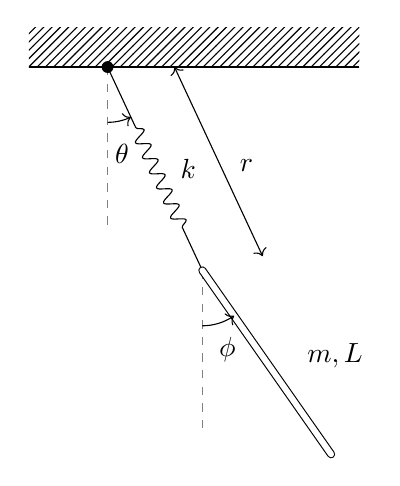
\begin{tikzpicture}

  \pgfmathsetmacro{\Gvec}{1.5}
  \pgfmathsetmacro{\myAngle}{25}

  \coordinate (centro) at (0,0);
  \draw[dashed,gray,-] (centro) -- ++ (0,-2) node (vert1) [black,below]{$ $};

  \draw (centro) -- ++(270+\myAngle:.85) coordinate (spring1);
  \draw[decorate, decoration={snake, segment length=6, amplitude=2.4}] (spring1) -- ++(270+\myAngle:1.5) coordinate (spring);
  \draw (spring) -- ++(270+\myAngle:.5) coordinate (spring2);
  \pic [draw,angle radius=20,->, "$\theta~$", angle eccentricity=1.6] {angle = vert1--centro--spring};

  \draw[<->] (.85,0) -- ++(270+\myAngle:2.65) coordinate (r);
  \draw ($(.85,0) + (270+\myAngle:2.75/2)$) node[label=0:$r$] {};
  \draw ($(.25,0) + (270+\myAngle:2.75/1.5)$) node[label=$k$] {};


  \fill[pattern = north east lines] ($(-1,0)$) rectangle ($(3.2,0.5) $);
  \draw[thick] ($ (centro) + (-1,0) $) -- ($ (centro) + (3.2,0) $);
\draw[dashed,gray,-] (spring2) -- ++ (0,-2) node (vert2) [black,below] {};
  \draw[double distance = .75mm,line cap=round] (spring2) -- ++(270+\myAngle+10:2.85) coordinate (bar);

  \draw ($ (bar) + (.05,1.25)$) node[label] {$m,L$};


  \pic [draw,angle radius=20,->, "$\phi$", angle eccentricity=1.5] {angle = vert2--spring2--bar};

  \fill[black] (centro) circle (0.075);
\end{tikzpicture}

\end{minipage}%
\begin{minipage}[c]{.6\textwidth}
  The pendulum system consists of a rigid bar pinned to the free end of a linear spring,
  which rotates about its opposite end at a fixed point; there are three degrees of freedom,
  since the spring and bar each have an individual angular deflection with respect to the vertical,
  and the radial distance the bar is from the point of rotation due to the variation in the
  length of the spring.
\end{minipage}
\end{figure}

\subsection{Constants and Assumptions}
\begin{tabular}{ll@{\hskip .75in}l}
 \multicolumn{1}{c}{Constants:} && \multicolumn{1}{c}{Assumptions:} \\
 Bar Mass: &$m$ = 1 kg & No Losses\\
 Bar Length: &$L$ = 1 m & Released from Rest\\
 Gravity: &$g$ = 9.81$\sfrac{m}{s^2}$ &Uniform Slender Bar \\
 Linear Spring: &&Planar\\
 \quad Spring Coefficient:& $k = 25~\sfrac{N}{m}$ &Rigid-Body Dynamics \\
 \quad Unstretched Length:& $L$ = 0.5 m \\
\end{tabular}
\vspace{5ex}

We are asked to determine the following: \\
\begin{enumerate}
  \item The Equations of Motion for the system via the Lagrangian method.
  \item Integrate the Equations of Motion using various initial conditions and plot
  the behavior of the system for 10 seconds. \\
  \vspace{2ex}
  $
  \begin{array}{cll}
    \text{(a)} & \theta_o = 0~rad, & \phi_o = 0~rad \\
    \text{(b)} & \theta_o = \sfrac{\pi}{18}~rad, & \phi_o = \sfrac{\pi}{9}~rad \\
    \text{(c)} & \theta_o = \sfrac{\pi}{6}~rad, & \phi_o = \sfrac{\pi}{3}~rad \\
  \end{array}
  $
  \item Plot the total energy versus time for all 3 cases.
  \item Repeat 2. and 3. using a '|RelTol|' of 1e-6 and '|AbsTol|' of 1e-9 for the
  |ode45| integration tolerances.
\end{enumerate}
\newpage
% ---------------------------------------------------------------------------- %
\section{Free Body Diagram}
% ---------------------------------------------------------------------------- %
\begin{figure}[!htp]
   \begin{minipage}[c]{.4\textwidth}
      
\begin{tikzpicture}

  \pgfmathsetmacro{\Gvec}{1.5}
  \pgfmathsetmacro{\myAngle}{25}

  \coordinate (centro) at (0,0);
  \draw[dashed,gray,-] (centro) -- ++ (0,-2) node (vert1) [black,below]{$ $};

  \draw (centro) -- ++(270+\myAngle:.85) coordinate (spring1);
  % \draw[decorate, gray, decoration={snake, segment length=6, amplitude=2.4}]
    % (spring1) -- ++(270+\myAngle:1.5) coordinate(spring);
  % \draw [gray] (spring) -- ++(270+\myAngle:.5) coordinate (spring2);
  \draw[decorate, decoration={snake, segment length=8, amplitude=2.1}]
    (spring1) -- ++(270+\myAngle:1.8) coordinate (springs);
  \draw (springs) -- ++(270+\myAngle:.5) coordinate (springs2);

  \pic [draw,angle radius=20,->, "$\theta~$", angle eccentricity=1.6] {angle = vert1--centro--spring};

  \draw [decorate,decoration={brace,amplitude=2pt,raise=4pt}] (0,0) --
    node [xshift=4.2ex,yshift=1.1ex] {$\ell_0 + \delta$} (springs2);

  % \draw[->] (.85,0) -- ++(270+\myAngle:2.65) coordinate (r);
  % \draw ($(.85,0) + (270+\myAngle:2.75/2)$) node[label=0:$r$] {};
  % \draw ($(.25,0) + (270+\myAngle:2.75/1.5)$) node[label=$k$] {};
  \path (centro) -- node[label={[label distance = 2ex]below:$k$}] (k) {} (spring2);

  \draw [gray,dashed] (-1,0) -- node[above,near end] (datum) {\textit{datum}} (2.5,0);
  \draw[dashed,gray,-] (springs2) -- ++ (0,-2) node (vert2) [black,below] {};
  \draw[double distance = .75mm,line cap=round] (springs2) -- ++(270+\myAngle+10:2.85) coordinate (bar);

  \pic [draw,angle radius=20,->, "$\phi$", angle eccentricity=1.5] {angle = vert2--spring2--bar};

  \coordinate (g) at ($(springs2) + (305:1.425)$);
  \path let \p1 = (g) in node at (\x1,0) (gdatum) {};
  \draw [dashed,gray,-] (g) -- (gdatum);
  \fill[black] (g) circle (0.03);

  % \begin{scope}[shift={(spring2)}]
  %   \draw[gray,dashed,domain=-30:-80] plot ({1.425*cos(\x)}, {1.425*sin(\x)});
  % \end{scope}

  \draw [decorate,decoration={brace,amplitude=2pt,raise=4pt,mirror}] (g) --
    node [xshift=4ex] {$V_{bar}$} (gdatum);

  \draw (g) node[label={[label distance = -1ex]225:$G$}] {};

  \fill[black] (centro) circle (0.075);
\end{tikzpicture}

   \end{minipage}%
   \begin{minipage}[c]{.6\textwidth}
     \center
     \begin{tabular}{rl}
     $G$:&Center of gravity of the bar\\
   \end{tabular}
   \end{minipage}
\end{figure}
% ---------------------------------------------------------------------------- %
\section{Coordinate Frame} \label{section:coord}
% ---------------------------------------------------------------------------- %
\begin{figure}[ht]
    \begin{minipage}[c]{.4\textwidth}
      \center
      \label{coord}
      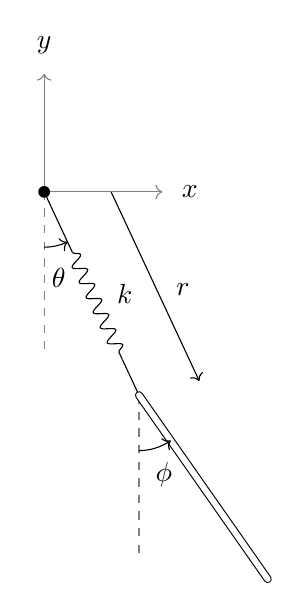
\begin{tikzpicture}

  \pgfmathsetmacro{\Gvec}{1.5}
  \pgfmathsetmacro{\myAngle}{25}

  \coordinate (centro) at (0,0);
  \draw[dashed,gray,-] (centro) -- ++ (0,-2) node (vert1) [black,below]{$ $};

  \draw (centro) -- ++(270+\myAngle:.85) coordinate (spring1);
  \draw[decorate, decoration={snake, segment length=6, amplitude=2.4}] (spring1) -- ++(270+\myAngle:1.5) coordinate (spring);
  \draw (spring) -- ++(270+\myAngle:.5) coordinate (spring2);
  \pic [draw,angle radius=20,->, "$\theta~$", angle eccentricity=1.6] {angle = vert1--centro--spring};

  \draw[->] (.85,0) -- ++(270+\myAngle:2.65) coordinate (r);
  \draw ($(.85,0) + (270+\myAngle:2.75/2)$) node[label=0:$r$] {};
  \draw ($(.25,0) + (270+\myAngle:2.75/1.5)$) node[label=$k$] {};

  \draw[gray,->] (0,0) -- ++ (1.5,0) node (x) {};
  \draw[gray,->] (0,0) -- ++ (0,1.5) node (y) {};
  \draw (x) node[label=east:$x$] {};
  \draw (y) node[label=north:$y$] {};

  \draw[dashed,gray,-] (spring2) -- ++ (0,-2) node (vert2) [black,below] {};
  \draw[double distance = .75mm,line cap=round] (spring2) -- ++(270+\myAngle+10:2.85) coordinate (bar);

  \pic [draw,angle radius=20,->, "$\phi$", angle eccentricity=1.5] {angle = vert2--spring2--bar};

  % \fill[black] ($(spring2) + (305:1.425)$) circle (0.03) coordinate (g);
  % \draw ($(spring2) + (320:1.425)$) node[label] {$G$};

  \fill[black] (centro) circle (0.075);
\end{tikzpicture}

      \caption{Coordinate Frame}
      \vspace{2ex}
    \end{minipage}%
    \begin{minipage}[c]{.6\textwidth}
      \center
      \begin{tabular}{rl}
      & \quad Motion Variables: \\
      $\theta$:& Angle of spring relative to vertical\\
      $\phi$:& Angle of bar relative to vertical\\
      $r$:& Radial length of spring \\
      \\
      & \quad Supplemental Variables: \\
      $\vec{r}_G$:& Vector to bar center of mass from origin \\
    \end{tabular}
    \end{minipage}
\end{figure}
% ---------------------------------------------------------------------------- %
\section{Sum of Forces}
% ---------------------------------------------------------------------------- %
% ---------------------------------------------------------------------------- %
\section{Constraints}
% ---------------------------------------------------------------------------- %
The system is fully constrained, therefore no constrain equations were needed to
solve the problem.
% ---------------------------------------------------------------------------- %
\section{Solve for the Equations of Motion}
% ---------------------------------------------------------------------------- %

\newpage
% ---------------------------------------------------------------------------- %
\section{Solve the Equations of Motion}
% ---------------------------------------------------------------------------- %
\begin{figure}[!htp]
  \caption{Numerical Solution Motion Behavior Plots, ($\theta_o:~0,~\phi_o:~0$)}
  \begin{subfigure}[t]{\textwidth}
  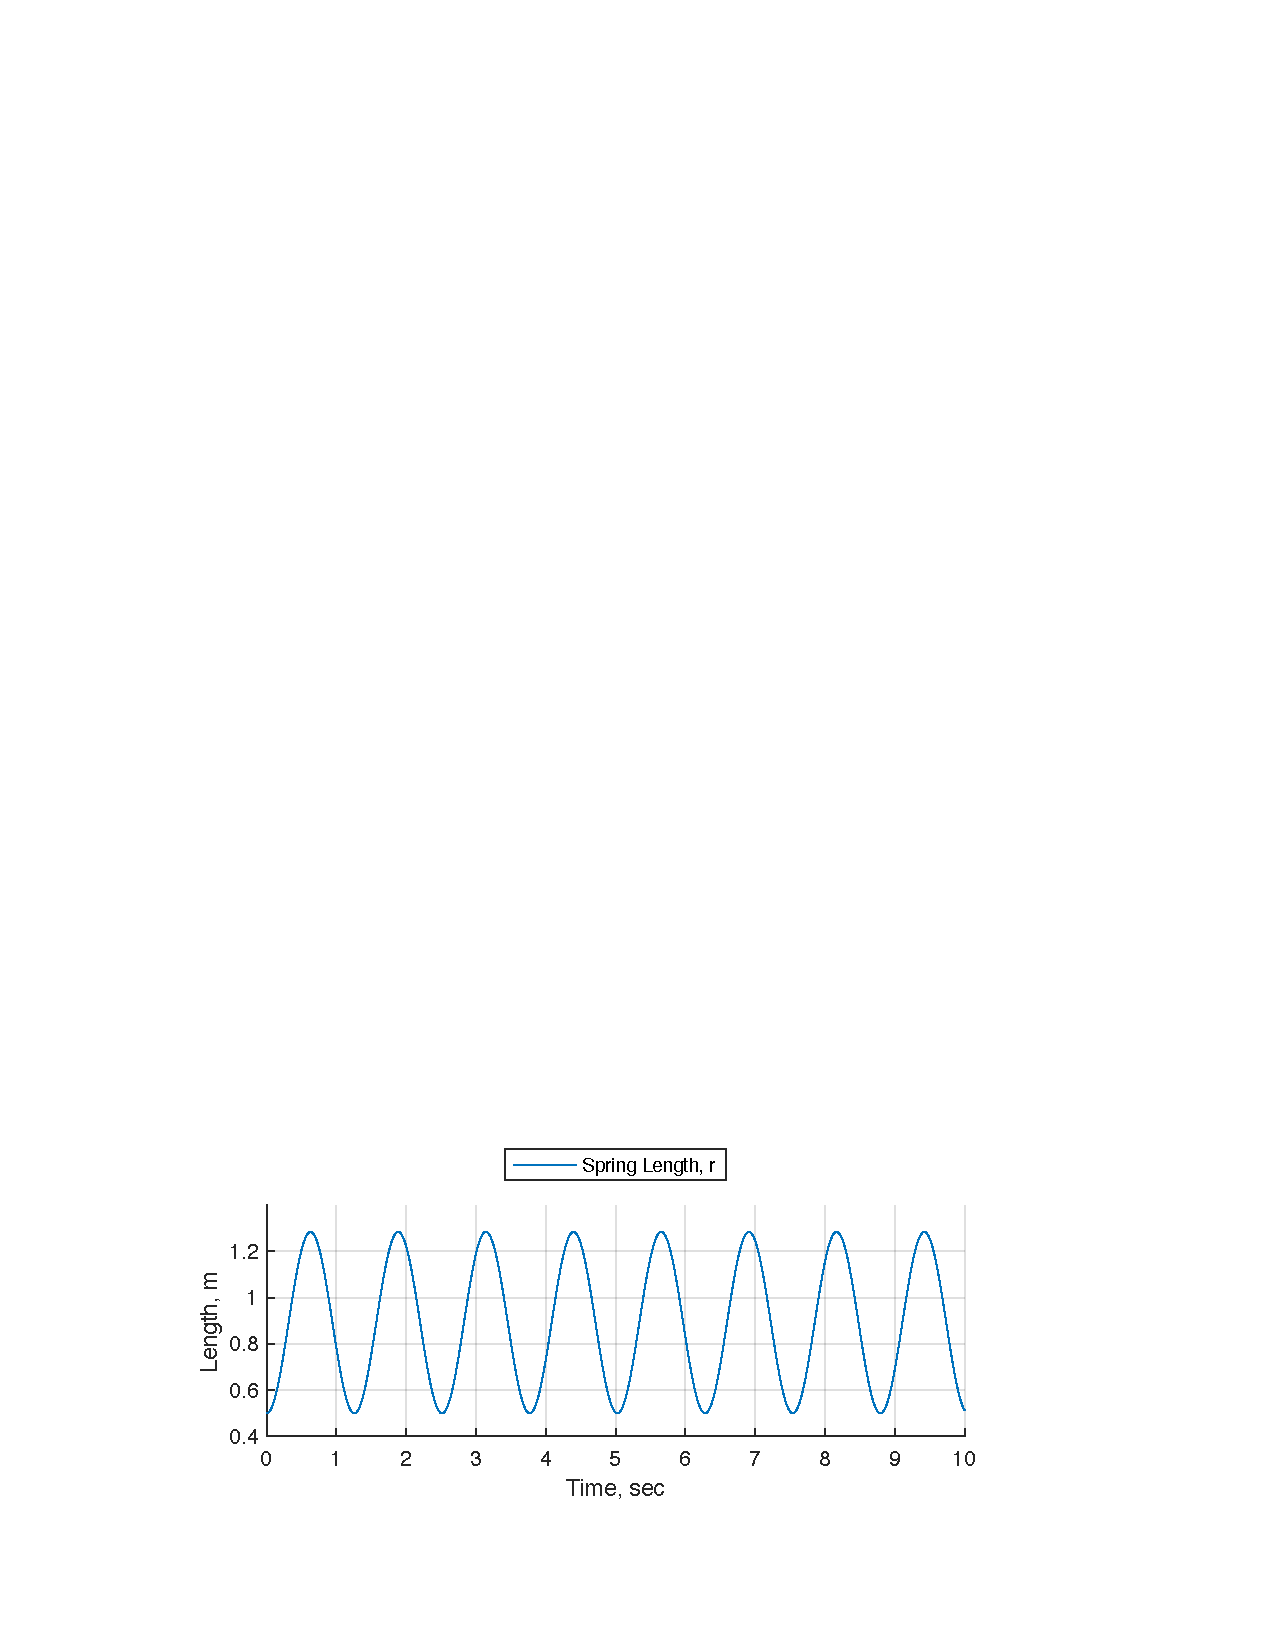
\includegraphics[center]{spring_0-0}
  \caption{Spring Length vs. Time}
  \label{fig:spring:0:0}
\end{subfigure}
\end{figure}

\begin{figure}[!htp]
  \caption{Numerical Solution Motion Behavior Plots, ($\theta_o:\sfrac{\pi}{18},~\phi_o:\sfrac{\pi}{9}$)}
\begin{subfigure}[t]{\textwidth}
  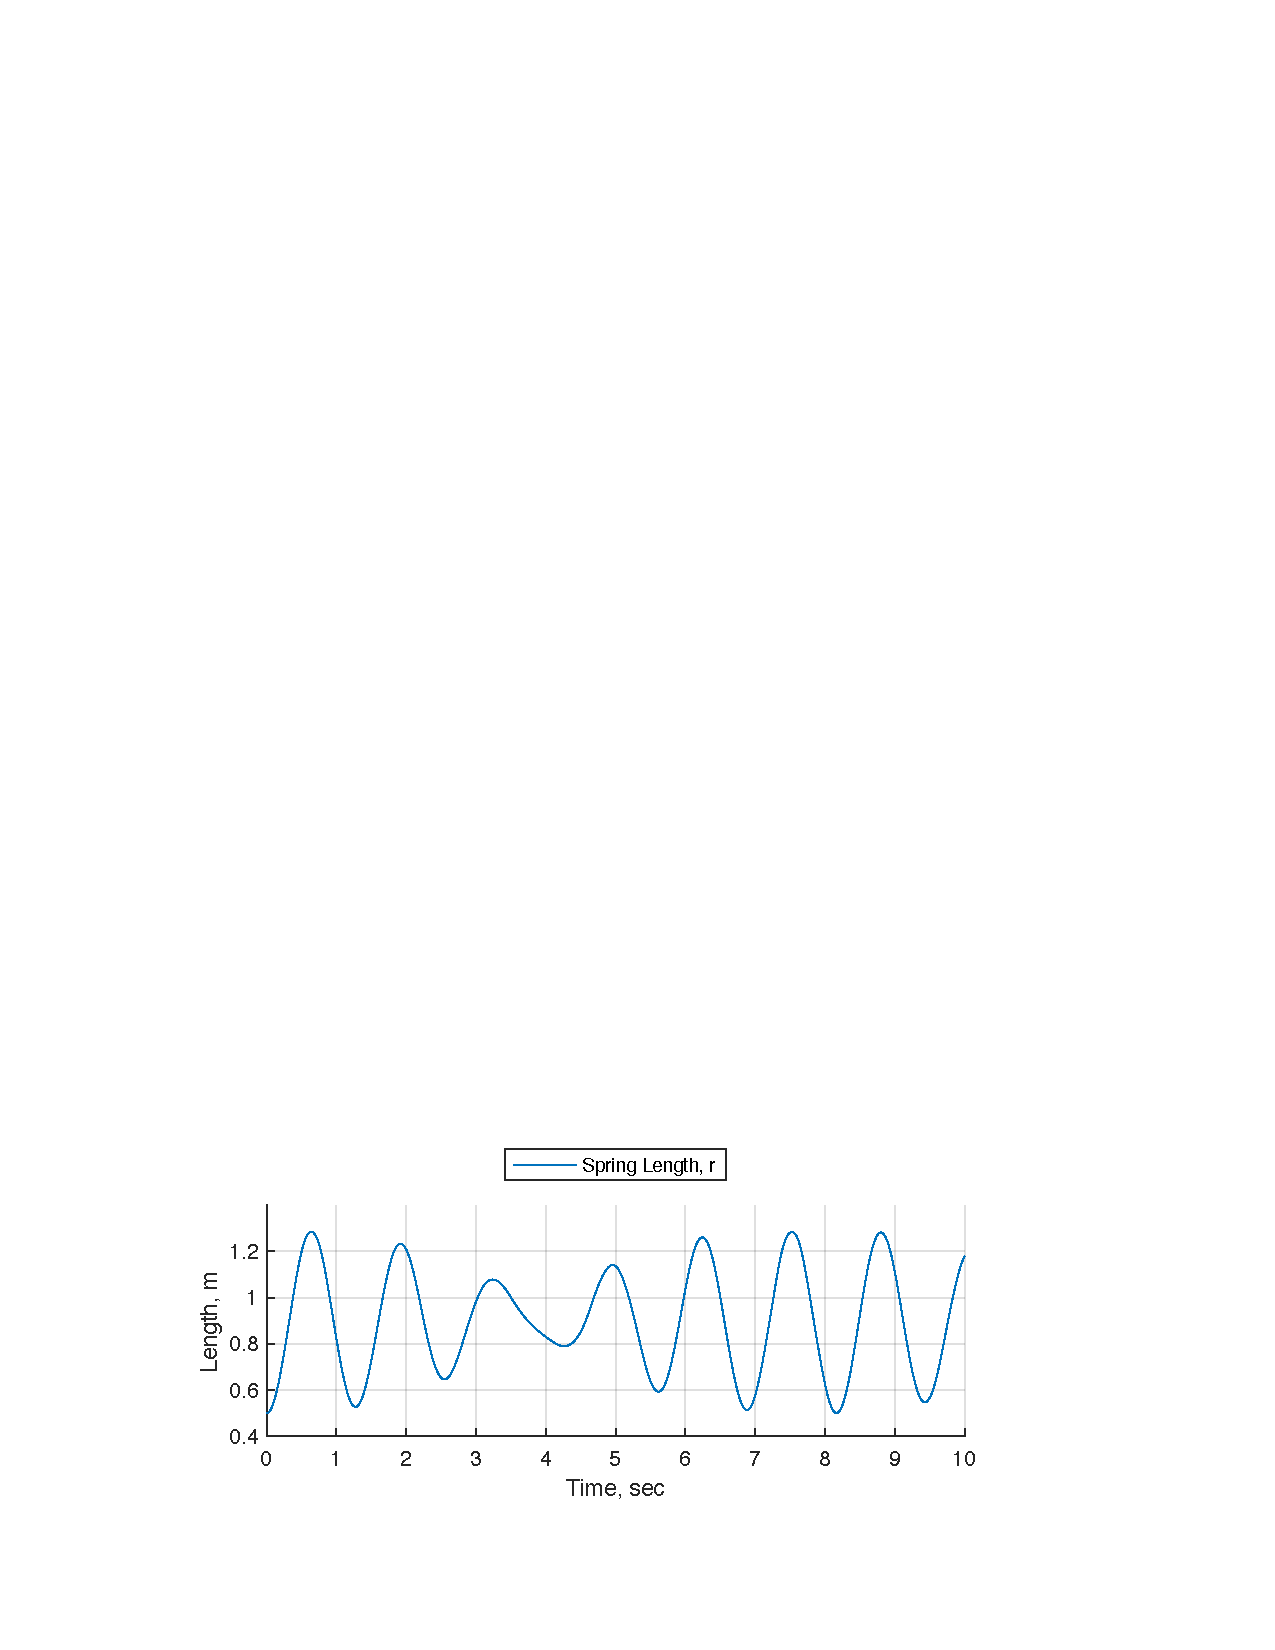
\includegraphics[center]{spring_18-9}
  \caption{Spring Length vs. Time}
  \label{fig:spring:18-9}
\end{subfigure}
\end{figure}

\begin{figure}[!htp] \ContinuedFloat
  \phantomcaption
\begin{subfigure}[t]{\textwidth}
  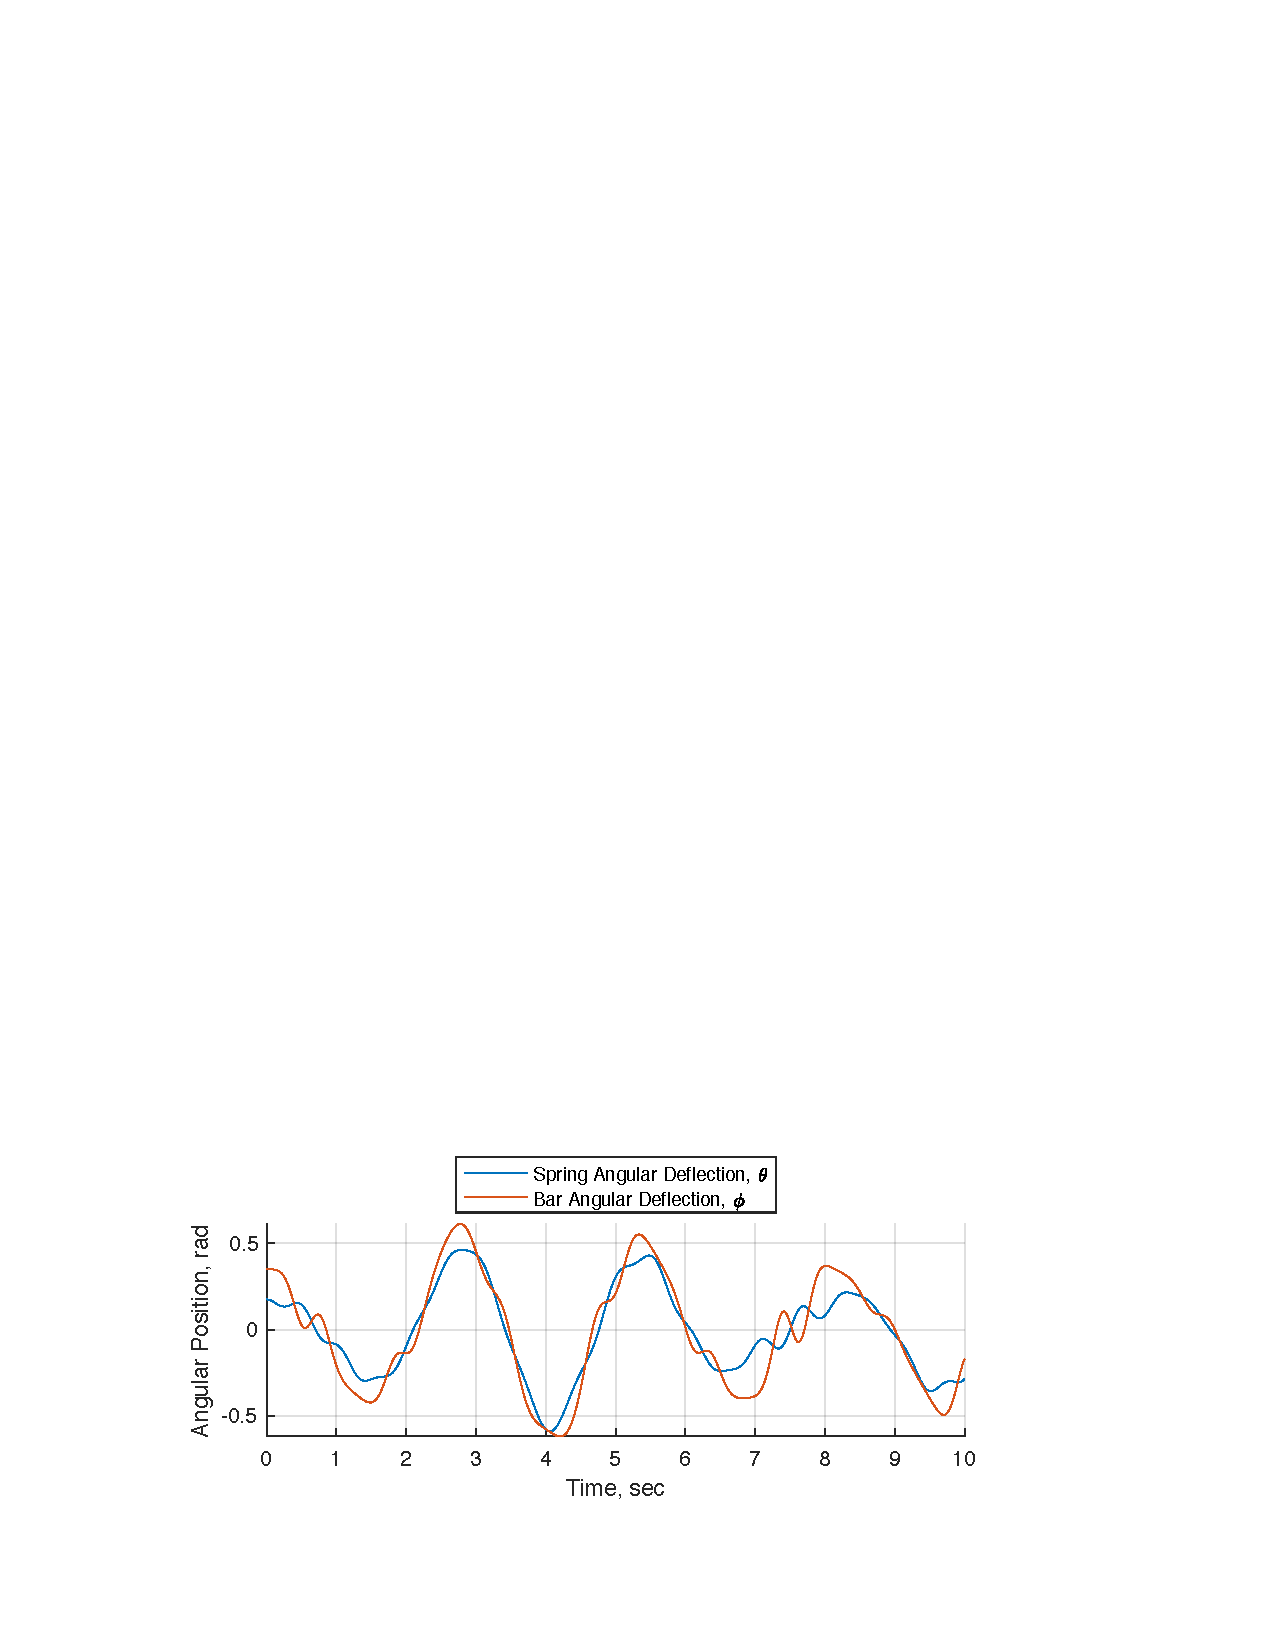
\includegraphics[center]{angles_18-9}
  \caption{Angular Position vs. Time}
  \label{fig:angles:18-9}
\end{subfigure}
\end{figure}

\begin{figure}[!htp]
  \caption{Numerical Solution Motion Behavior Plots, ($\theta_o:\sfrac{\pi}{6},~\phi_o:\sfrac{\pi}{3}$)}
\begin{subfigure}[t]{\textwidth}
  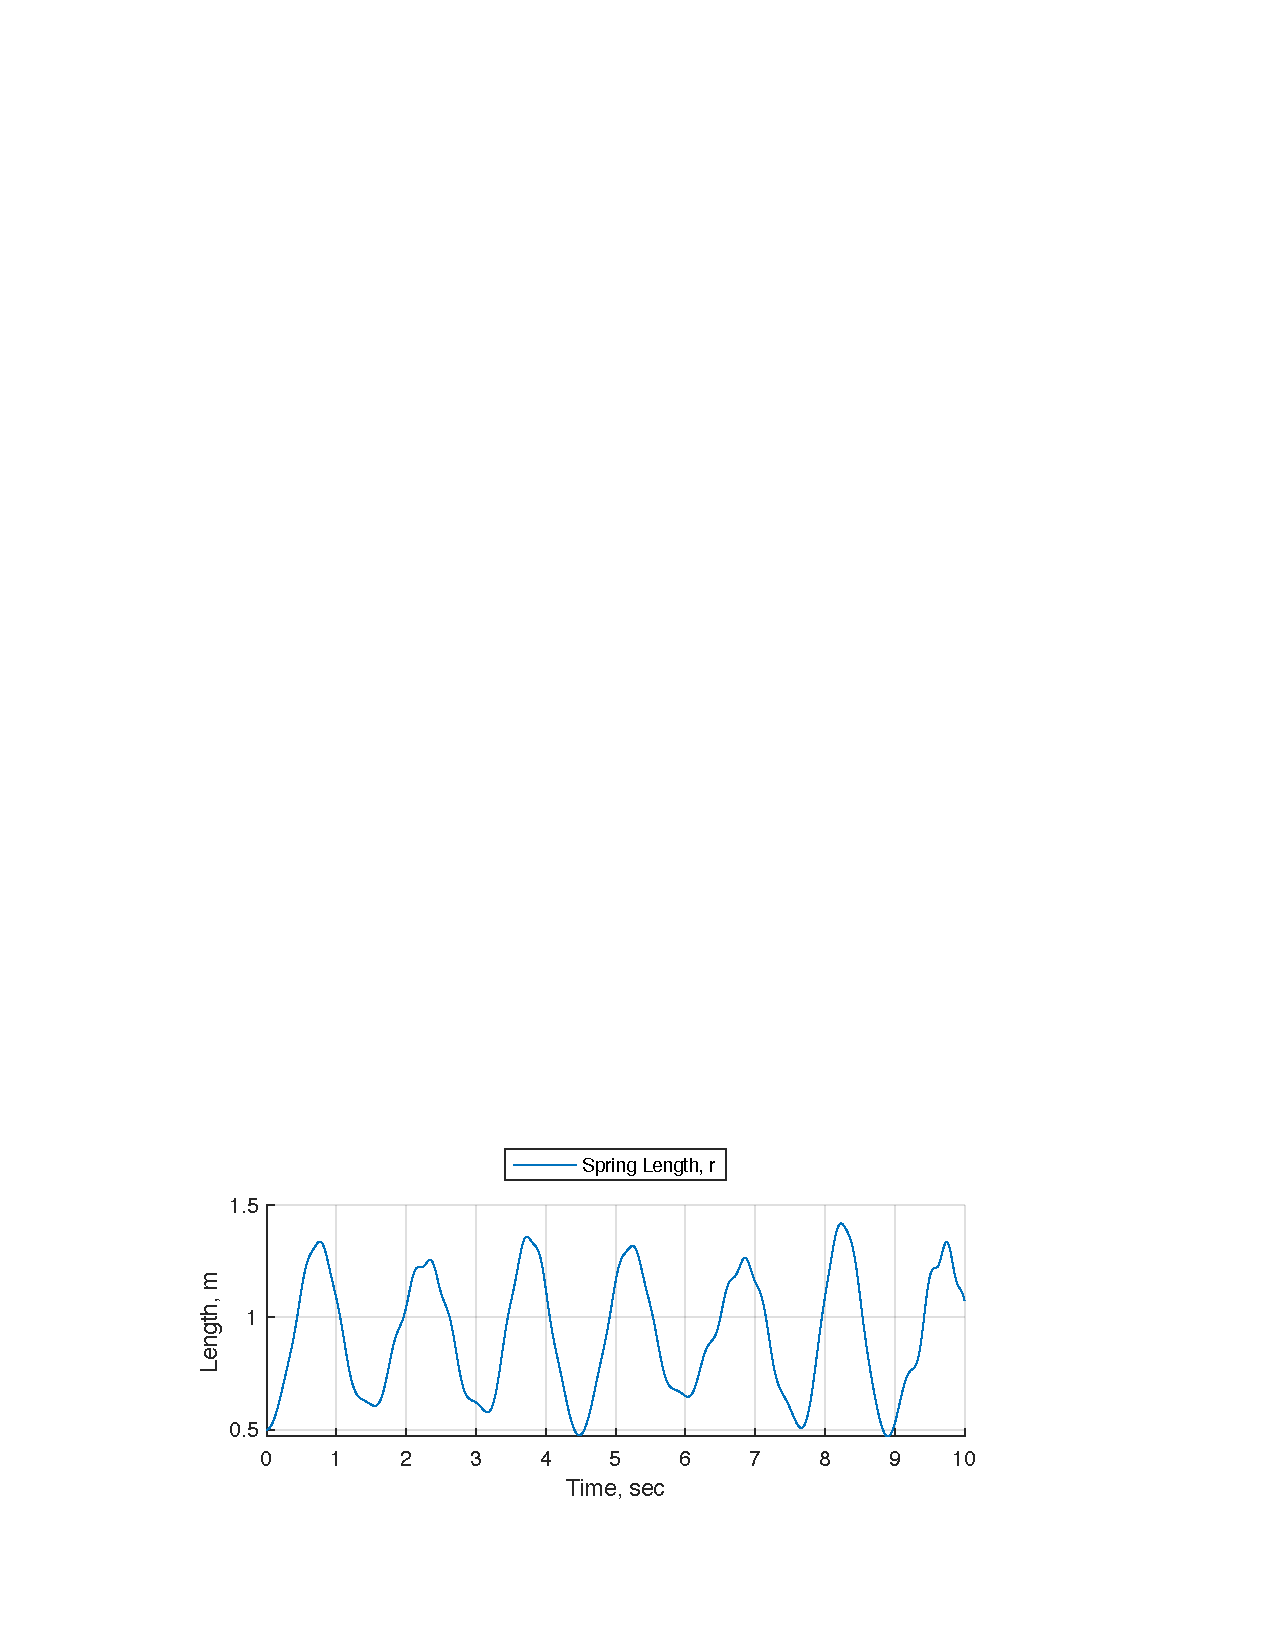
\includegraphics[center]{spring_6-3}
  \caption{Spring Length vs. Time}
  \label{fig:spring:6-3}
\end{subfigure}
\end{figure}

\begin{figure}[!htp] \ContinuedFloat
  \phantomcaption
\begin{subfigure}[t]{\textwidth}
  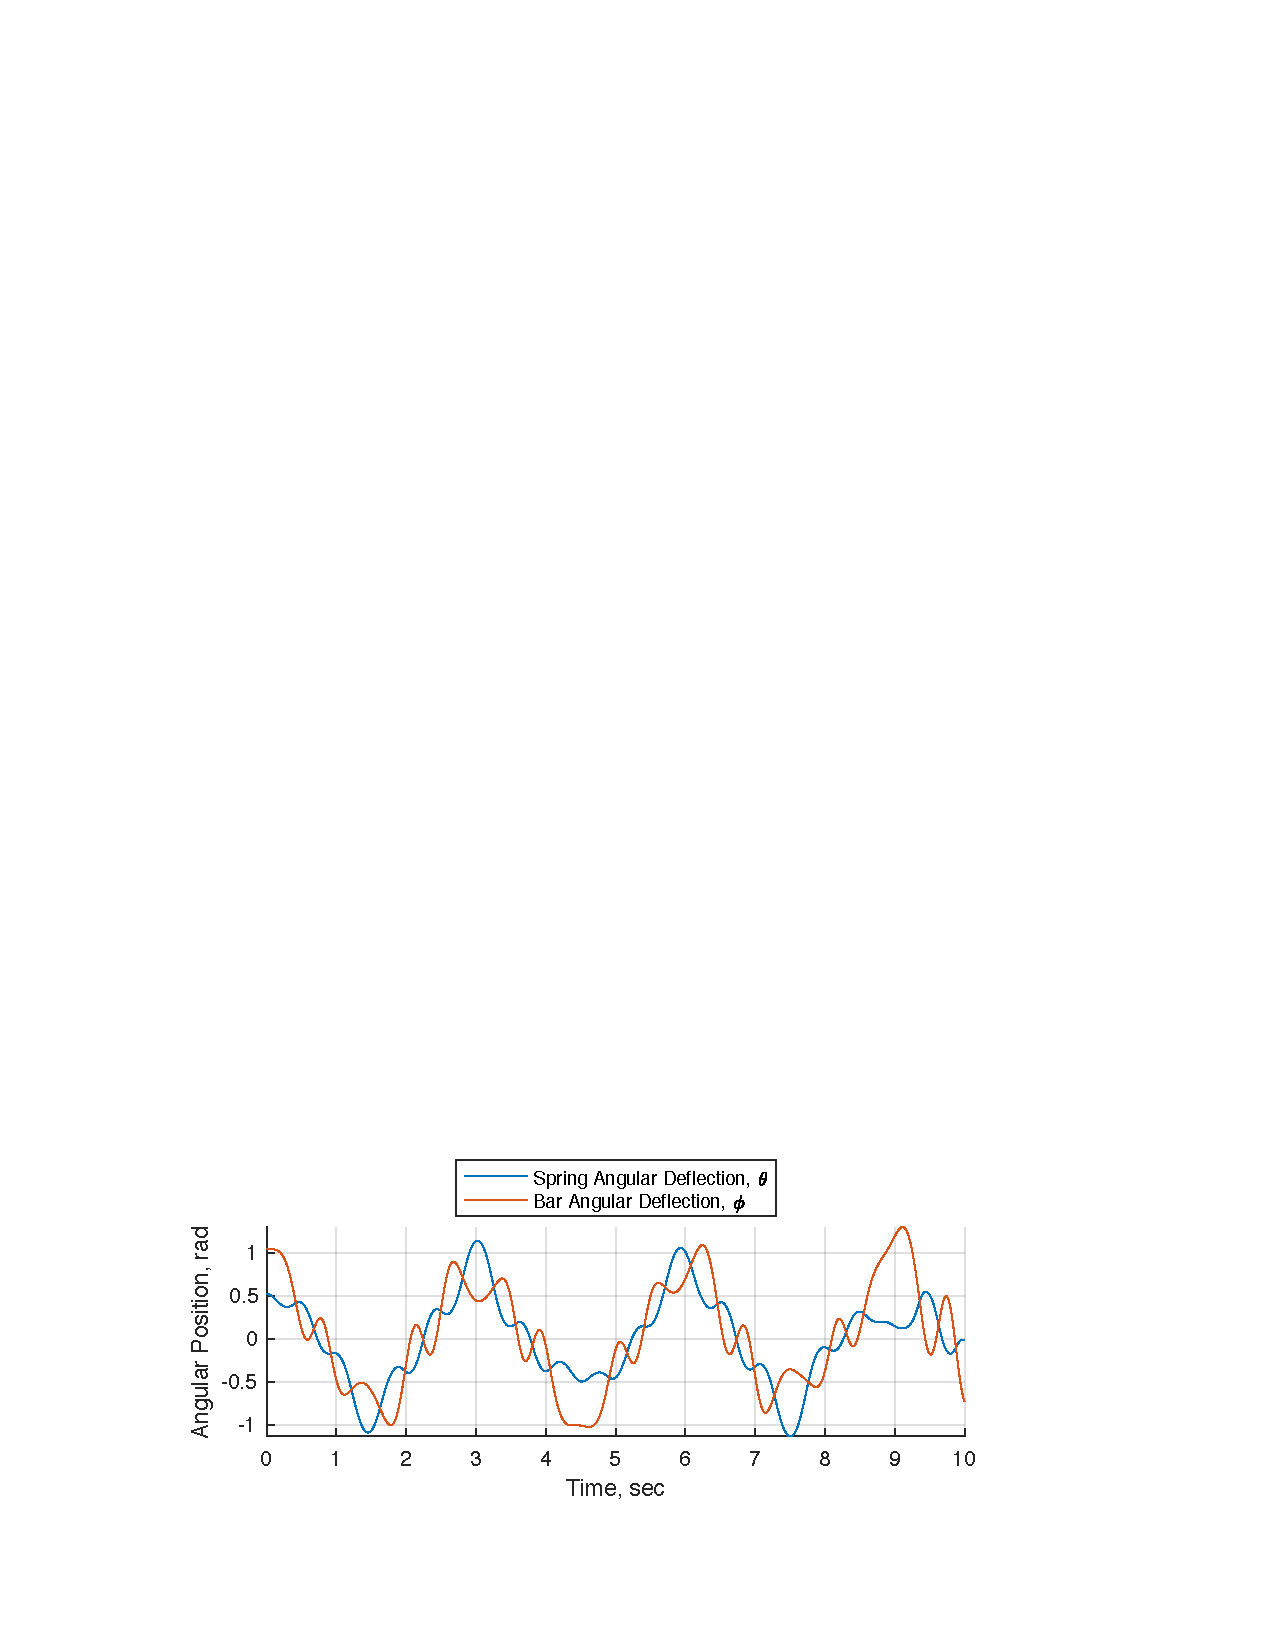
\includegraphics[center]{angles_6-3}
  \caption{Angular Position vs. Time}
  \label{fig:angles:6-3}
\end{subfigure}
\end{figure}

% ---------------------------------------------------------------------------- %
\section{Does it Make Sense?}
% ---------------------------------------------------------------------------- %
\subsection{Units}
Checking with the MATLAB symbolic units tool (from Section \ref{appendix:numerical}): \\
~\\
% \begin{lstlisting}[frame=lines,style=Matlab-editor]
% Checking EOM Units
u = symunit;
m2 = m2*u.kg;
k = k*u.N/u.m;
L0 = L0*u.m;
l2 = l2*u.m;
g = g*u.m/u.s^2;
thetat = 'thetat';
thetadot = 'thetadot'/u.s;
thetaddot = 'thetaddot'/u.s^2;
phit = 'phit';
phidot = 'phidot'/u.s;
phiddot = 'phiddot'/u.s^2;
l1t = 'l1t'*u.m;
l1dot = 'l1dot'*u.m/u.s;
l1ddot = 'l1ddot'*u.m/u.s^2;

eqn = subs(eqn)
unitCheck = checkUnits(eqn)
\end{lstlisting}
\color{gray} \begin{verbatim}
unitCheck =
  struct with fields:
    Consistent: [1 1 1]
    Compatible: [1 1 1]
\end{verbatim} \color{black}

\subsection{Magnitude}

\section{Appendix} \label{appendix}
\subsection{Attributions}
\onehalfspacing
\begin{tabular}{ll}
Jeffrey Chen & \\
Thorne Wolfenbarger &\\
Trey Dufrene & \\
Joint Effort &
\end{tabular}
\singlespacing

\newpage
\subsection{Analytical Solution}

\newpage
\subsection{Numerical Solution} \label{appendix:numerical}
% \begin{lstlisting}[frame=lines,style=Matlab-editor,basicstyle = \mlttfamily]

\end{lstlisting}


\end{flushleft}
\end{document}
